% TEMPLATE.TEX
%
% Time-stamp: <2013-03-26 11:09 olenz>
%
% This is an extensively documented LaTeX file that shows how to
% produce a good-looking document with current LaTeX (11/2012).
%
% IMPORTANT!
%
%   Some obsolete commands and packages
% ----------|-------------------------------
% obsolete  |     Replacement in LATEX 2ε
% ----------|-------------------------------
%           | local            global/switch
% ----------|-------------------------------
% {\bf ...} | \textbf{...}     \bfseries
%     -     | \emph{...}       \em
% {\it ...} | \textit{...}     \itshape
%     -     | \textmd{...}     \mdseries
% {\rm ...} | \textrm{...}     \rmfamily
% {\sc ...} | \textsc{...}     \scshape
% {\sf ...} | \textsf{...}     \sffamily
% {\sl ...} | \textsl{...}     \slshape
% {\tt ...} | \texttt{...}     \ttfamily
%     -     | \textup{...}     \upshape
%
% DON'T USE \\ TO MAKE LINEBREAKS, INSTEAD JUST LEAVE A BLANK LINE!
%
\RequirePackage[l2tabu,orthodox]{nag} % turn on warnings because of bad style
\documentclass[a4paper,10pt,bibtotoc]{scrartcl}
%
\usepackage[bottom=3.5cm, top=2cm]{geometry}
%%%%%%%%%%%%%%%%%%%%%%%%%%%%%%%%%%%%
% KOMA CLASSES
%%%%%%%%%%%%%%%%%%%%%%%%%%%%%%%%%%%%
%
% The class "scrartcl" is one of the so-called KOMA-classes, a set of
% very well done LaTeX-classes that produce a very European layout
% (e.g. titles with a sans-serif font).
%
% The KOMA classes have extensive documentation that you can access
% via the commands:
%   texdoc scrguide # in German
%   texdoc scrguien # in English
%
%
% The available classes are:
%
% scrartcl - for "articles", typically for up to ~20 pages, the
%            highest level sectioning command is \section
%
% scrreprt - for "reports", typically for up to ~200 pages, the
%            highest level sectioning command is \chapter
%
% scrbook  - for "books", for more than 200 pages, the highest level
%            sectioning command is \part.
%
% USEFUL OPTIONS
%
% a4paper  - Use a4 paper instead of the default american letter
%            format.
%
% 11pt, 12pt, 10pt
%          - Use a font with the given size.
%
% bibtotoc - Add the bibliography to the table of contents
%
% The KOMA-script classes have plenty of options to modify

% This allows to type UTF-8 characters like ä,ö,ü,ß
\usepackage[utf8]{inputenc}

\usepackage[T1]{fontenc}        % Tries to use Postscript Type 1 Fonts for better rendering
\usepackage{lmodern}            % Provides the Latin Modern Font which offers more glyphs than the default Computer Modern
\usepackage[intlimits]{amsmath} % Provides all mathematical commands

\usepackage{hyperref}           % Provides clickable links in the PDF-document for \ref
\usepackage{graphicx}            % Allow you to include images (like graphicx). Usage: \includegraphics{path/to/file}

% Allows to set units
\usepackage[ugly]{units}        % Allows you to type units with correct spacing and font style. Usage: $\unit[100]{m}$ or $\unitfrac[100]{m}{s}$

% Additional packages
\usepackage{url}                % Lets you typeset urls. Usage: \url{http://...}
\usepackage{breakurl}           % Enables linebreaks for urls
\usepackage{xspace}             % Use \xpsace in macros to automatically insert space based on context. Usage: \newcommand{\es}{ESPResSo\xspace}
\usepackage{xcolor}             % Obviously colors. Usage: \color{red} Red text
\usepackage{booktabs}           % Nice rules for tables. Usage \begin{tabular}\toprule ... \midrule ... \bottomrule

% Source code listings
\usepackage{listings}           % Source Code Listings. Usage: \begin{lstlisting}...\end{lstlisting}
\lstloadlanguages{python}
\definecolor{lightpurple}{rgb}{0.8,0.8,1}

\lstset{
stepnumber=1,
numbersep=5pt,
numberstyle=\small\color{black},
basicstyle=\ttfamily,
%keywordstyle=\color{black},
%commentstyle=\color{black},
%stringstyle=\color{black},
frame=single,
tabsize=4,
language = python,
backgroundcolor=\color{black!5}}

\usepackage{float}

\begin{document}

\titlehead{Simulation Methods in Physics II \hfill SS 2020}
\title{Report for Worksheet 1: Calculate solid crystalline materials using density functional theory}
\author{Markus Baur and David Beyer}
\date{\today}
\maketitle

\tableofcontents

\section{Short Questions --Short Answers}
\begin{itemize}
 \item A1: 
 \item A2:
 \item A3:
 \item A4:
 \item A5:
\end{itemize}


\section{Quantum Mechanical Calculations using CP2K}
The following section deals with DFT-calculatiosn for diamond.

\subsection{Converging the Cutoff Energy}
In order to find an appropriate cutoff energy, we ran calculations with different values of the cutoff energy (between 50 and 450 Rydberg). REL\_CUTOFF was set to 60 Rydberg. \autoref{fig:fig1} shows the computed total energies as a function of the cutoff energy. We can clearly see that the total energy sharply decreases when the cutoff energy is increased from 50 Ry to 100 Ry. However, a further increase in the cutoff energy does not change much. Because of this, we used a cutoff energy of 100 Ry in the following simulations.

\begin{figure}[h]
\centering
 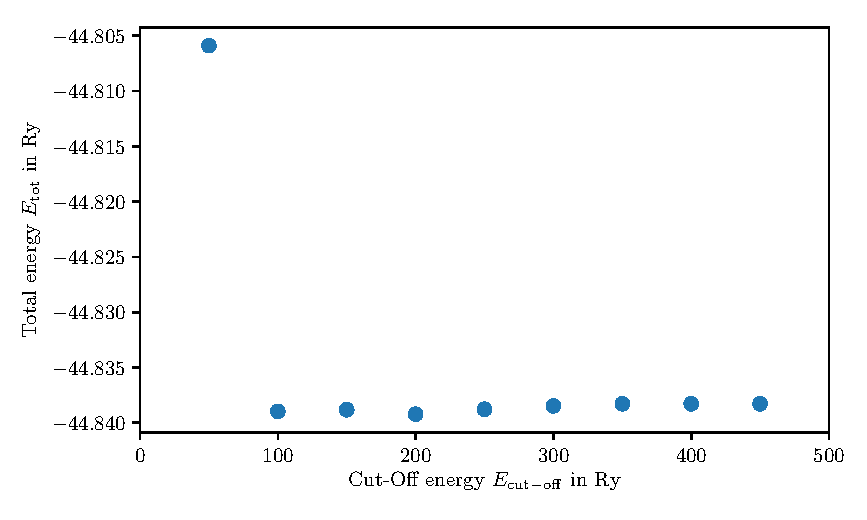
\includegraphics[width=\textwidth]{Figure_cutoff_energy.pdf}
 \caption{Plot of the calculated total energy for different cutoff energies.}
 \label{fig:fig1}
\end{figure}

\subsection{Optimzing the Lattice Constant}
To optimize the crystal structure, we ran calculations with the RUN\_TYPE GEO\_OPT and different values of the lattice constant. We could then determine the equilibirium lattice constant using a fit.

\subsubsection{PBE Functional}
\autoref{fig:fig2} shows the calculated total energy as a function of the volume $V=a^3$ of the unit cell. It is easy to see that there is a minimum. In order to determine the corresponding equilibrium volume, we fitted the quadratic function
\begin{align}
f(V) = a + b\cdot\left(V-V_\mathrm{eq}\right)^2
\end{align}
to the calculated values, this is also shown in the plot. The obtained fit parameters are
\begin{align}
a &= -44.9809763\,\mathrm{Ry}\\
b &= 7.72048911\cdot 10^{-4}\,\frac{\mathrm{Ry}}{\r{A}^9}\\
V_\mathrm{eq} &= 50.7015415\,\r{A}^3.
\end{align}
The equilibrium volume can be calculated from $V_\mathrm{eq}$ and is given by
\begin{align}
a_\mathrm{eq} = \sqrt[3]{V_\mathrm{eq}} \approx 3.70\,\r{A}.
\end{align}
This value is about 3\% larger than the experimental value of $a_\mathrm{eq,exp.} \approx 3.57\,\r{A}$\footnote{http://lampx.tugraz.at/~hadley/ss1/crystalstructure/structures/diamond/diamond.php, accessed on April 30, 2020 at 22:00}, which means that PBE overestimates the lattice constant.

\autoref{fig:fig3} shows a visualization of the primitive unit cell of diamond which was created using the software VMD (Visual Molecular Dynamics). The structure was taken from the simulation with the equilibrium lattice constant.


\begin{figure}[h]
\centering
 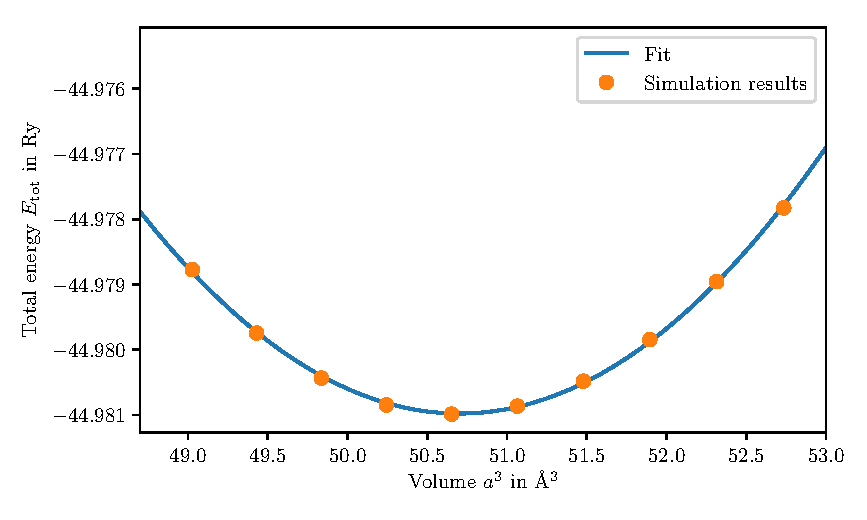
\includegraphics[width=\textwidth]{Figure_lattice_constant_PBE.pdf}
 \caption{Plot of the calculated total energy (using the PBE functional) as a function of the volume of the unit cell. The fit-function which is also shown is a parabola which was fitted to the obtained values in order to determine the equilibrium lattice constant.}
 \label{fig:fig2}
\end{figure}

\begin{figure}[h]
\centering
 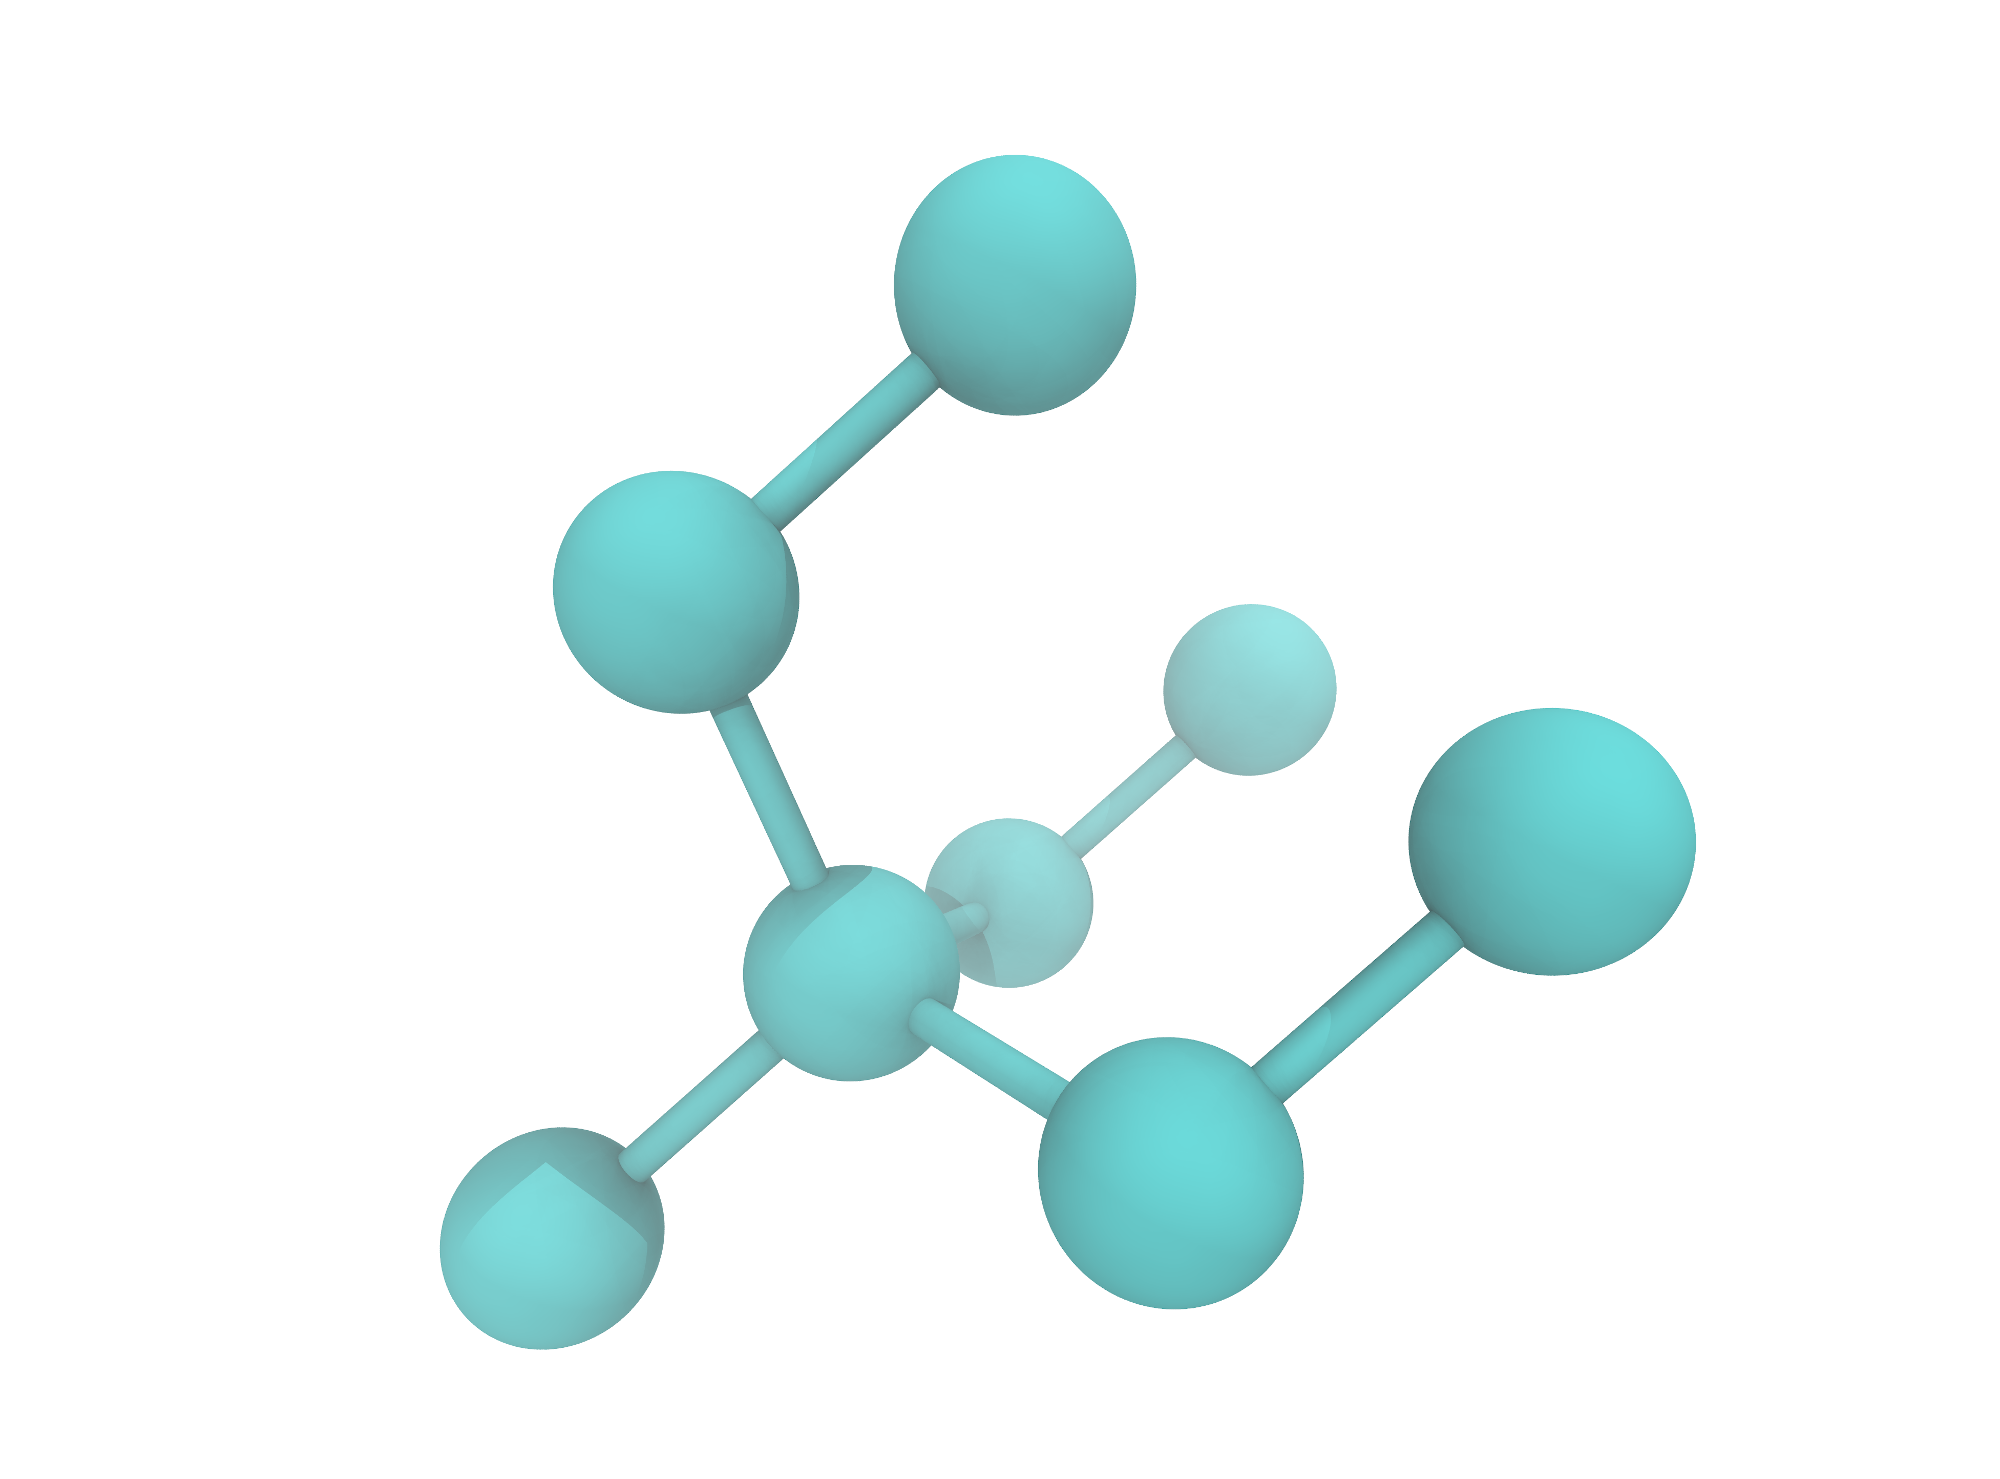
\includegraphics[width=\textwidth]{structure.png}
 \caption{Visualization of the crystal structure of diamond. The shown selection corresponds to the primite unit cell.}
 \label{fig:fig3}
\end{figure}

\subsubsection{LDA Functional}

\subsection{Electronic Structure Calculation}

\end{document}
